\section{Hardware}

Hardware (HW) omfatter systemet fra sensor til nettverksprotokollen som blir brukt i
bilsystemet. Hvilken HW
som trengs er da avhengig av noen faktorer:
\begin{itemize}
\item Tilgjengelige sensorer.
\item Format av nettverksdata.
\item Nødvendig dataprosessering.
\item Utfordringer ved signaloverføring.
\item Bruk av nettverksprotokoll.
\end{itemize}

Dette delkapittelet vil gå nærmere inn på faktorene som er med på å definere og begrense HW design. I tillegg
studeres ulike krav sensorteknologier stiller til HW. Til slutt sammenlignes ulike HW design.

%hvilke sensorer som er tilgjengelige, hvilke data
%man får fra de ulike sensorene, hvilken dataprosessering som er nødvendig og
%utfordringer i forhold til signaloverføring og
%hvilken nettverksprotokoll som brukes. \\

\subsection{Definerende og begrensende faktorer}

En definerenede faktor for HW er måleteknikk. Det er da særlig krets
mellom eventuelt mikrokontroller (MCU) og sensor som vil variere. Ulike måleteknikker studeres
i kapittel \ref{subsec:sensorteknologier}. Måleteknikken setter også en begrensing på hva som er
mulig å måle og dermed hvilke tjenester systemet kan tilby. 

I bilindustrien er CAN den rådende nettverksprotokollen \cite{canbus}. Man
kan argumentere for at man på grunnlag av dette burde integrere nye systemer på
det eksisterende nettverket. Uansett hvilket nettverk det skal kommuniseres over
vil det stille krav til HW. En ny enhet bør ha riktig nettverksgrensesnitt
og må kunne kommunisere på riktig protokoll. 

\subsection{Sensorteknologier}
\label{subsec:sensorteknologier}

Det er flere fysiske prinsipper som kan måles for å detektere en løs hjulmutter.
Det er derfor viktig å undersøke hvilke sensorteknologier som er tilgjengelig og
hvilke fordeler disse drar med seg. Tre ulike fysiske prinsipper som kan brukes er strekk, trykk og vibrasjon. 

\subsubsection{Vibrasjonsmåling}

Vibrasjonsmåling kan bli gjort med teknologier som et akselerometer eller ved
pizoelektriske mikrofoner. Slike sensorer vil kunne gi et signal som inneholder
ulike frekvenstyper som kan analyseres. Slik kan man gjenkjenne mønstre i
frekvensbåndet som indikerer eksempevis en løs mutter. For å analysere dette signalet må det
samples med en Analog-til-Digital Converter (ADC) \cite{adc}. Dersom signalet er svakt må det også forsterkes gjennom en
forsterker krets. 

For å hente ut informasjon av signalet må en algoritme undersøke
frekvensoppbyggingen av signalet. Dette kan bli gjort i HW med en Digital Signal Processor (DSP) \cite{dsp}, men kan
også gjøres i software (SW) ved at det sendes en signalprøve fra HW til kontrolsystemet. Å
bruke en DSP kompliserer HW og effektforbruk og kost øker. Det krever også at algoritmen på DSP'en 
er lastet inn før den brukes og kan ikke endres uten at den omprogrammeres. Analyseres signalene i HW kan vil
det kunne sendes korte datapakker på CAN bussen og sampling av signalet vil kunne gjøres kontinuerlig. Dette er
positivt med tanke på å ikke overbelaste CAN bussen som brukes av mange andre enheter i bilen. 

Analyserer man signalet i SW blir det lettere å oppdatere algoritmen etter installasjon av HW
samt at det kan benyttes artificial intellegence (AI) til å justere algoritmen bassert på målinger underveis. 
Dette forenkler HW litt ved at man ikke trenger en DSP krets, men HW blir nødt å sende større pakker over CAN
bussen. Dette kan potensielt bruke opp båndbredden til CAN bussen dersom store pakker med data sendes ofte. 
Det er vitkig å komme frem til en akseptabel størrelse på samplingsdataen som skal sendes samt frekvensen på
sendingen. Dette avgjøres i storgrad av den eksisterende trafikken på CAN bussen.

%Tanken er å ha sensoren på akslingen mellom to hjul. For å skille mellom hvilket
%hjul som har løse muttere, så kan det være en løsning å bruke en sensor ved vært
%hjul. Da er to mulig algoritmer å måle amplitudeforskjell eller
%tidsforsinkelse. Dette burde være mulig å få til med en MCU, men kan være det
%blir nødvendig med en DSP for raskere prosessering av signalene. \\
%
%MCUen sender pakkene med en ID slik at man kan skille mellom ulike akslinger. \\

\subsubsection{Strekklapper/Trykklapper}

Strekklapper og trykklapper, som illustrert i figur \ref{fig:Strekklapp_vector} og \ref{fig:Trykklapp_vector} baserer seg på samme prinsipp ved at det gir ut et målbart signal avhengig av
motstandsendringen i lappen. 
\begin{figure}[H] \centering
\subfigure[]{
	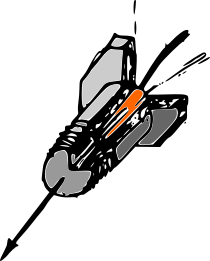
\includegraphics[width=0.2 \textwidth]{images/Straingage_vector.png}
	\label{fig:Strekklapp_vector}
	}
\hspace{3cm}
\subfigure[]{
	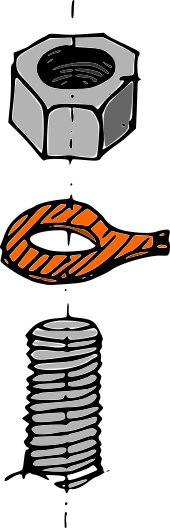
\includegraphics[width=0.1 \textwidth]{images/trykklapp_vector.png}
	\label{fig:Trykklapp_vector}
	}
\caption{\protect{\ref{fig:Strekklapp_vector}} Strekklapp i bolt (orange), \protect{\ref{fig:Trykklapp_vector}} Trykklapp (orange) mellom bolt og mutter.}
\end{figure}
Ved å legge strekklapper inni eller på utsiden av boltene eller
trykklapper mellom mutter og nav kan det detekteres om en mutter løsner. Strekklappene
legges i en wheatstone bridge \cite{wheatstone} for å kunne gi ut et målbart
spenningsnivå. For å oppnå et målbart spenningsnivå kan det kreves å
forsterke signalet gjennom en forsterker krets. Denne analoge målingen krever mye lavere sampling enn ved
vibrasjonsmålinger da det trengs kortere signalprøver.
% problemer med at signalet fra strekklappen må gjennom en slepering.
%Dette kan by på utfordringer med tanke på implementasjon og støy.
Det kreves også ha en sensor per bolt. Dette kompliserer HW, men en måte å redusere
mengden HW på kan være å multiplexe signalene fra hver sensor til MCU'en. 
%Det er mulig å lage
%en krets hvor man benytter seg av tidskonstanten i en RC-krets (dette må du
%undersøke litt). 
Overføring av signaler fra nav til aksling kan også skje ved induksjon. 
%For å koble til flere
%enheter på et CAN bus så kan man benytte seg av J1939 som fordelere ID på
%nettverket (dette må du undersøke litt mer). \\

\subsection{Utfordringer}

Problemet med å måle vibrasjoner er at en sampleprøve av et signal innenfor et gitt tidsrom kan bli veldig stor. Som
et resultat at de store sampleprøvene kan det oppstå båndbreddeproblemer på CAN-bussen. Grunnen til dette
er at samplingsfrekvensen man sampler signalet med må være
minst dobbelt så høy som frekvensen av signalet, i følge Nyquist–Shannon sampling theorem \cite{nyquist}. Høyere
samplingsrate gir bedre signalrepresentasjon, og en god
representasjon av signalet kan være viktig for en eventuell analysealgoritme.

Dersom analysealgoritmen kjøres på en DSP slipper CAN-bussen og overbelastes av store datamengder.
Algoritmen ligger ikke da i det sentrale systemet og det kan bli vanskeligere å forbedre algoritmen ved hjelp av AI. 
